\documentclass[
	a4paper, % Paper size, specify a4paper (A4) or letterpaper (US letter)
	12pt, % Default font size, specify 10pt, 11pt or 12pt
]{class}

\addtolength{\textwidth}{1.75in}
\addtolength{\oddsidemargin}{-.850in}
\addtolength{\evensidemargin}{-.850in}

\usepackage{caption}
\usepackage{soul}
\usepackage{subcaption}

\addbibresource{bibliography.bib} % Bibliography file (located in the same folder as the template)
\nocite{*} 
%----------------------------------------------------------------------------------------
%	REPORT INFORMATION
%----------------------------------------------------------------------------------------

\title{GPU Computing Project\\Parallel implementation of Dijkstra's Algorithm} % Report title

\author{Tricella Davide 08361A} % Author name(s), add additional authors like: '\& James \textsc{Smith}'

\date{\today} % Date of the report

%----------------------------------------------------------------------------------------

\begin{document}

\maketitle % Insert the title, author and date using the information specified above

\begin{center}
    \begin{tabular}{l r}
        Instructor: Professor \textsc{Grossi Giuliano}
    \end{tabular}
\end{center}

%----------------------------------------------------------------------------------------
%	ABSTRACT
%----------------------------------------------------------------------------------------

\begin{abstract}
    The purpose of this paper is to describe the implementation and benchmarking of various parallel implementations of Dijkstra's Algorithm to solve the all-pairs shortest path problem.
\end{abstract}

%----------------------------------------------------------------------------------------
%	TOC
%----------------------------------------------------------------------------------------

\tableofcontents
\newpage
%----------------------------------------------------------------------------------------
%	INTRODUCTION
%----------------------------------------------------------------------------------------

\section{Introduction}

The problem of shortest path in a graph consists in finding the path, from node A to node B,
which minimizes the sum of edges weights of which the path is composed.\\

\begin{center}
    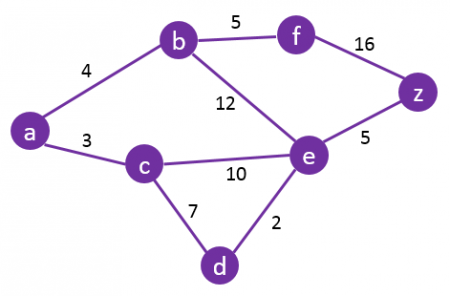
\includegraphics[width=10cm]{/images/graph.png}
    \captionof{figure}{Graph with edge weights}
\end{center}

In particular, the algorithm used for this document aim to solve the all-pairs shortest path problem,
which consists of finding the lenght of the shortest path for all the pairs of nodes.\\

The algorithm assumes that there are not negative weights and that the graph is undirected without isolated parts.\\

This problem is tackled in a lot of practical applications, like road networks path-finding, telecommunication routing and robot navigation.

\section{Dijkstra’s algorithm overview}
To solve the problem introduced before, there are several solutions which have been studied and improved troughout the years.
The option chosen for this task has been the Dijkstra’s algorithm, which has been implemented using the paper \cite{paper}
as a guidance.\\

This is a very well known algorithm, initially designed at the end of the 1950's, and used in a huge number of different applications.

The first version implemented was basically a parallel extension of the sequential algorithm,
then a more advanced approach has been taken for the improved version.

\newpage
\subsection{Sequential Version}
The basic algorithm solve the problem of shortest path between one Source Node and all the other nodes. The sequential version uses a for loop
to launch this version on every node of the graph, so at the end of the loop every node possesses the shortest path to every other node.\\

The main elements used during the computation are:\\
\begin{itemize}
    \item Graph Adiacency Matrix: which represents the graph indicating the weight of the edge which connects a node to another
    \item Vt Set: used as a stop condition and to check if a node has already a minimal path assigned
    \item l Array: which contains the minimal paths found for a certain node at a certain moment\\
\end{itemize}

We can divide the procedure into two main passages:\\
\begin{itemize}
    \item Initialization
    \item Main loop\\
\end{itemize}

During the first phase the Vt set is created containing only the Source Node, then the l Array is initialized, with the direct connections
from the Source Node to every other node, putting a symblic value of "infinity" where a direct connection is not available.\\

The the main loop begins, and continues until all the nodes are present in the Vt set. The Main cycle, is composed of two internal phases:\\
\begin{itemize}
    \item Local minimum search: between the elements of l not included in Vt we look for the minimum weight. Then we add the node selected to Vt.
    \item Update loop: the value of l, corresponding to the node selected before, gets updated with the minimum between the current value and the sum
    between the value selected during the minimum search and the weight present in the matrix. This part verifies if the value calculated by the search
    brings to a path actually shorter than the one stored.\\
\end{itemize}

When the Vt set is equal to the set of nodes of the graph, the Main loop terminates and the algorithm returns the l Array, 
where all the shortest paths are stored.\\

To solve the all pairs Shortest Paths problem we add an external loop that launch the algorithm for every row of the original Adiacency Matrix,
and at the end returns a new matrix, composed of the various l arrays computed for every node.

\subsubsection{Complexity}
The sequential algorithm perform $n$ times the basic algorithm , which has a complexity of O($n^2$):\\

\begin{itemize}
    \item Time per Source: $O(n^2)$
    \item Number of executions: $n$
    \item Total Time: $O(n^3)$\\
\end{itemize}

\subsection{Basic parallel version}
The idea behind the initially implemented parallel version is simple:
to solve the problem we have to launch the algorithm |V| times, where V is the set of nodes of the graph.
Every thread executes the algorithm for one node of the graph, and at the end insert the results in the correct
row of the matrix in Global Memory.\\

The computation has been spreaded over the gpu blocks using a fixed amount of threads per block (1024) and
a variable size of blocks, based on the number of nodes of the graph. \\

The shared memory is not used because the variables needed for the computation are all locally present inside the thread, which is the main advantage of
this first technique, because there are not requirements of any kind on inter-process communications. Each thread works completely isolated from the others.\\

Due to thread memory limitations, the main variables of each thread had to be stored into Global Memory, and retrieved using the global thread id, calculated
at the start of the computation.\\

This implementation requires a thread per node of the graph, which still uses the various for loops present in the sequential version,
this fact make this implementation simple to program, with a decent speedup, provided the graph is big enough.\\
The main problem is that it is not taking full advantage of the Gpu capabilities, which is the weak spot that the second version tries to address.

\subsubsection{Complexity}
This version improves the performance by performing the basic algorithm in parallel, and has no communication delay:\\
\begin{itemize}
    \item Time per Source: $O(n^2)$
    \item Number of executions: $1$
    \item Total Time: $O(n^2)$\\
\end{itemize}

\subsection{Improved parallel version}
This version aim to exploit more the parallel execution of the GPU, using one Block per node of the graph, and one thread for every node to evaluate in the block.
To reach this objective it is necessary to use the shared memory to save the varius data used during the computation of a block.\\

This time the threads are not isolated and need to cooperate to compute the final array for the block result.
The inner for loop now implement a Parallel reduction procedure which compute the local minimum of a node.\\

There are some critical section of the code, like the stop condition check, that have been assigned exclusively to the first thread of the block,
using the thread syncronization directive, because these steps are complex to parallelize, and the istruction executed by multiple threads could
cause concurrent acces which would slow down the evaluation.

\subsubsection{Complexity}
The improved version increases the concurrency by using $n$ processor per instance, so $n^2$ processors, this means thath every instance is executed
by n processors, but we have to take into account the communication delay:\\
\begin{itemize}
    \item Time per Source: $O(n^2/p + nlog(p))$
    \item Number of processors: $n$
    \item Total Time: $O(n^3 / n) + O(nlog(p)) = O(n^2) + O(nlog(p))$\\
\end{itemize}

\newpage
\section{Implementation details}

\subsection{Sequential version}
The sequential version is implemented by the function

\begin{verbatim}
    void shortestPathsSequential(int* matrix, int dimension, int* results)
\end{verbatim}

where matrix and results are respectively the Adiacency Matrix of the graph and the result matrix, while dimension is the number
of nodes of the graph.\\

Despite the fact that a matrix is generally considered a sparse and inefficient storage method for a graph, in this particular case this data structure
has the advantage of containing some vital information in the structure itself, while the same implementation of Dijkstra using a linked list type of structure 
would have been a lot more convoluted, with various auxilary implementations required to evalutate the weight of the path from every node to another.\\

It also would not make a lot of sense to encode the result of this algorithm into a listed structure, beacuse the objective is to find the path form very node to every other node,
so a list would not be as efficient as a matrix to encode $nodes^2$ values.\\

The data structures for the computation are then allocated and initialized, with Vt having all false values except for the Source node
and l having the values of the corresponding matrix row.
\begin{verbatim}
    bool* Vt = (bool*)malloc((dimension) * sizeof(bool));
    int* l = (int*)malloc(dimension * sizeof(int));
\end{verbatim}

The main loop start, using a simple function which check the Vt array as a stop condition
\begin{verbatim}
bool allTrue(bool* vector, int dimension)
\end{verbatim}

The search for the local minimum is executed.
\begin{verbatim}
for (int i = 0; i < dimension; i++) {
    if (Vt[i] == true) continue;
    if (l[i] < closestWeigth) {
        closestWeigth = l[i];
        closestIndex = i;
    }
}
\end{verbatim}

Then the Vt cell of the closest node is set to true and the l array is updated with the minimum between the current value and the
possible better value.
\begin{verbatim}
Vt[closestIndex] = true;
for (int i = 0; i < dimension; i++) {
    if (Vt[i] == true) continue;
    int uvWeight = matrix[closestIndex * dimension + i];
    l[i] = min(l[i], l[closestIndex] + uvWeight);
}
\end{verbatim}

When the main loop stops, the result matrix is filled with the values from the l array
\begin{verbatim}
for (int i = 0; i < dimension; i++) {
    results[node * dimension + i] = l[i];
}
\end{verbatim}

\subsection{Basic parallel version}
This simple parallel version is implemented by the function
\begin{verbatim}
__global__ void shortestPathsParallel(int* matrix, int dimension, int* results, int* lArray, bool* VtArray)
\end{verbatim}

The algorithm is not substantially different from the sequential version, the only change present is that now the reference for the
Source node is not the index of a for loop, but the calculated thread Id.\\

Every thread computes the sequential version without communicating in any way with other threads, not even during
the results copying section.

This means that during initialization the Vt index to set is the one corresponding to the idx variable. This id is also used during the
update of the l array and the filling of the results matrix.\\

\subsection{Improved parallel version}
The last version is implemented by the function
\begin{verbatim}
__global__ void shortestPathsParallelV2(int* matrix, int* results)
\end{verbatim}

This time the code has various significant differences from the sequential one.\\

Beginning from the initialization phase, the usage of multiple blocks required the utilization of the shared memory, to guarantee to all threads of the block
the necessary information with good access speed.
\begin{verbatim}
    // Shared memory initialization
    extern __shared__ int s[];
    int* sharedData = s;
    
    // l vector initialization
    int* l = (int*)&sharedData[0];
    
    // minimum vectors initialization
    int* minimumValues = (int*)&l[bDim];
    int* minimumIndexes = (int*)&minimumValues[bDim];
    
    // Boolean vector simulating the Vt set initialization
    bool* Vt = (bool*)&minimumIndexes[bDim];
    
    bool* stopCycle = (bool*)&Vt[bDim];
\end{verbatim}

The shared memory initialization contains an additional vector, the minimumValues and minimumIndexes arrays, used during the computation of the local minimum,
the first containing the weight of a certain node, the second containing the index of that node according to the original matrix.\\

This is necessary for the correct computation of the parallel reduction, because the standard reduction does not take into account an external index, which is necessary
in this application, so there are two assignments instead of one, one for the value, the other for the index.

\subsubsection{Parallel Reduction}
The Parallel Reduction is a strategy to perform quickly some operations that ouptut a single value from the computing of an array of values.
The idea is to maximize the usage of a parallel processor, by reducing the original array in smaller and smaller parts, with each thread evaluating two values per cycle.
At the end of the operation the result will lay in the first cell of the array.\\

This operation dows not require additional data structures to function, so it works competely in-place. The general field of application are mathematical operations such as sum or, in this case, a
minimum operation.

The standard algorithm of the reduction has been slighly modified to keep track of the node original index between the various passages. This comes with an additional
cost, because now the number of comparisons that a thread must perform for every cycle is two instead of one.


\begin{center}
    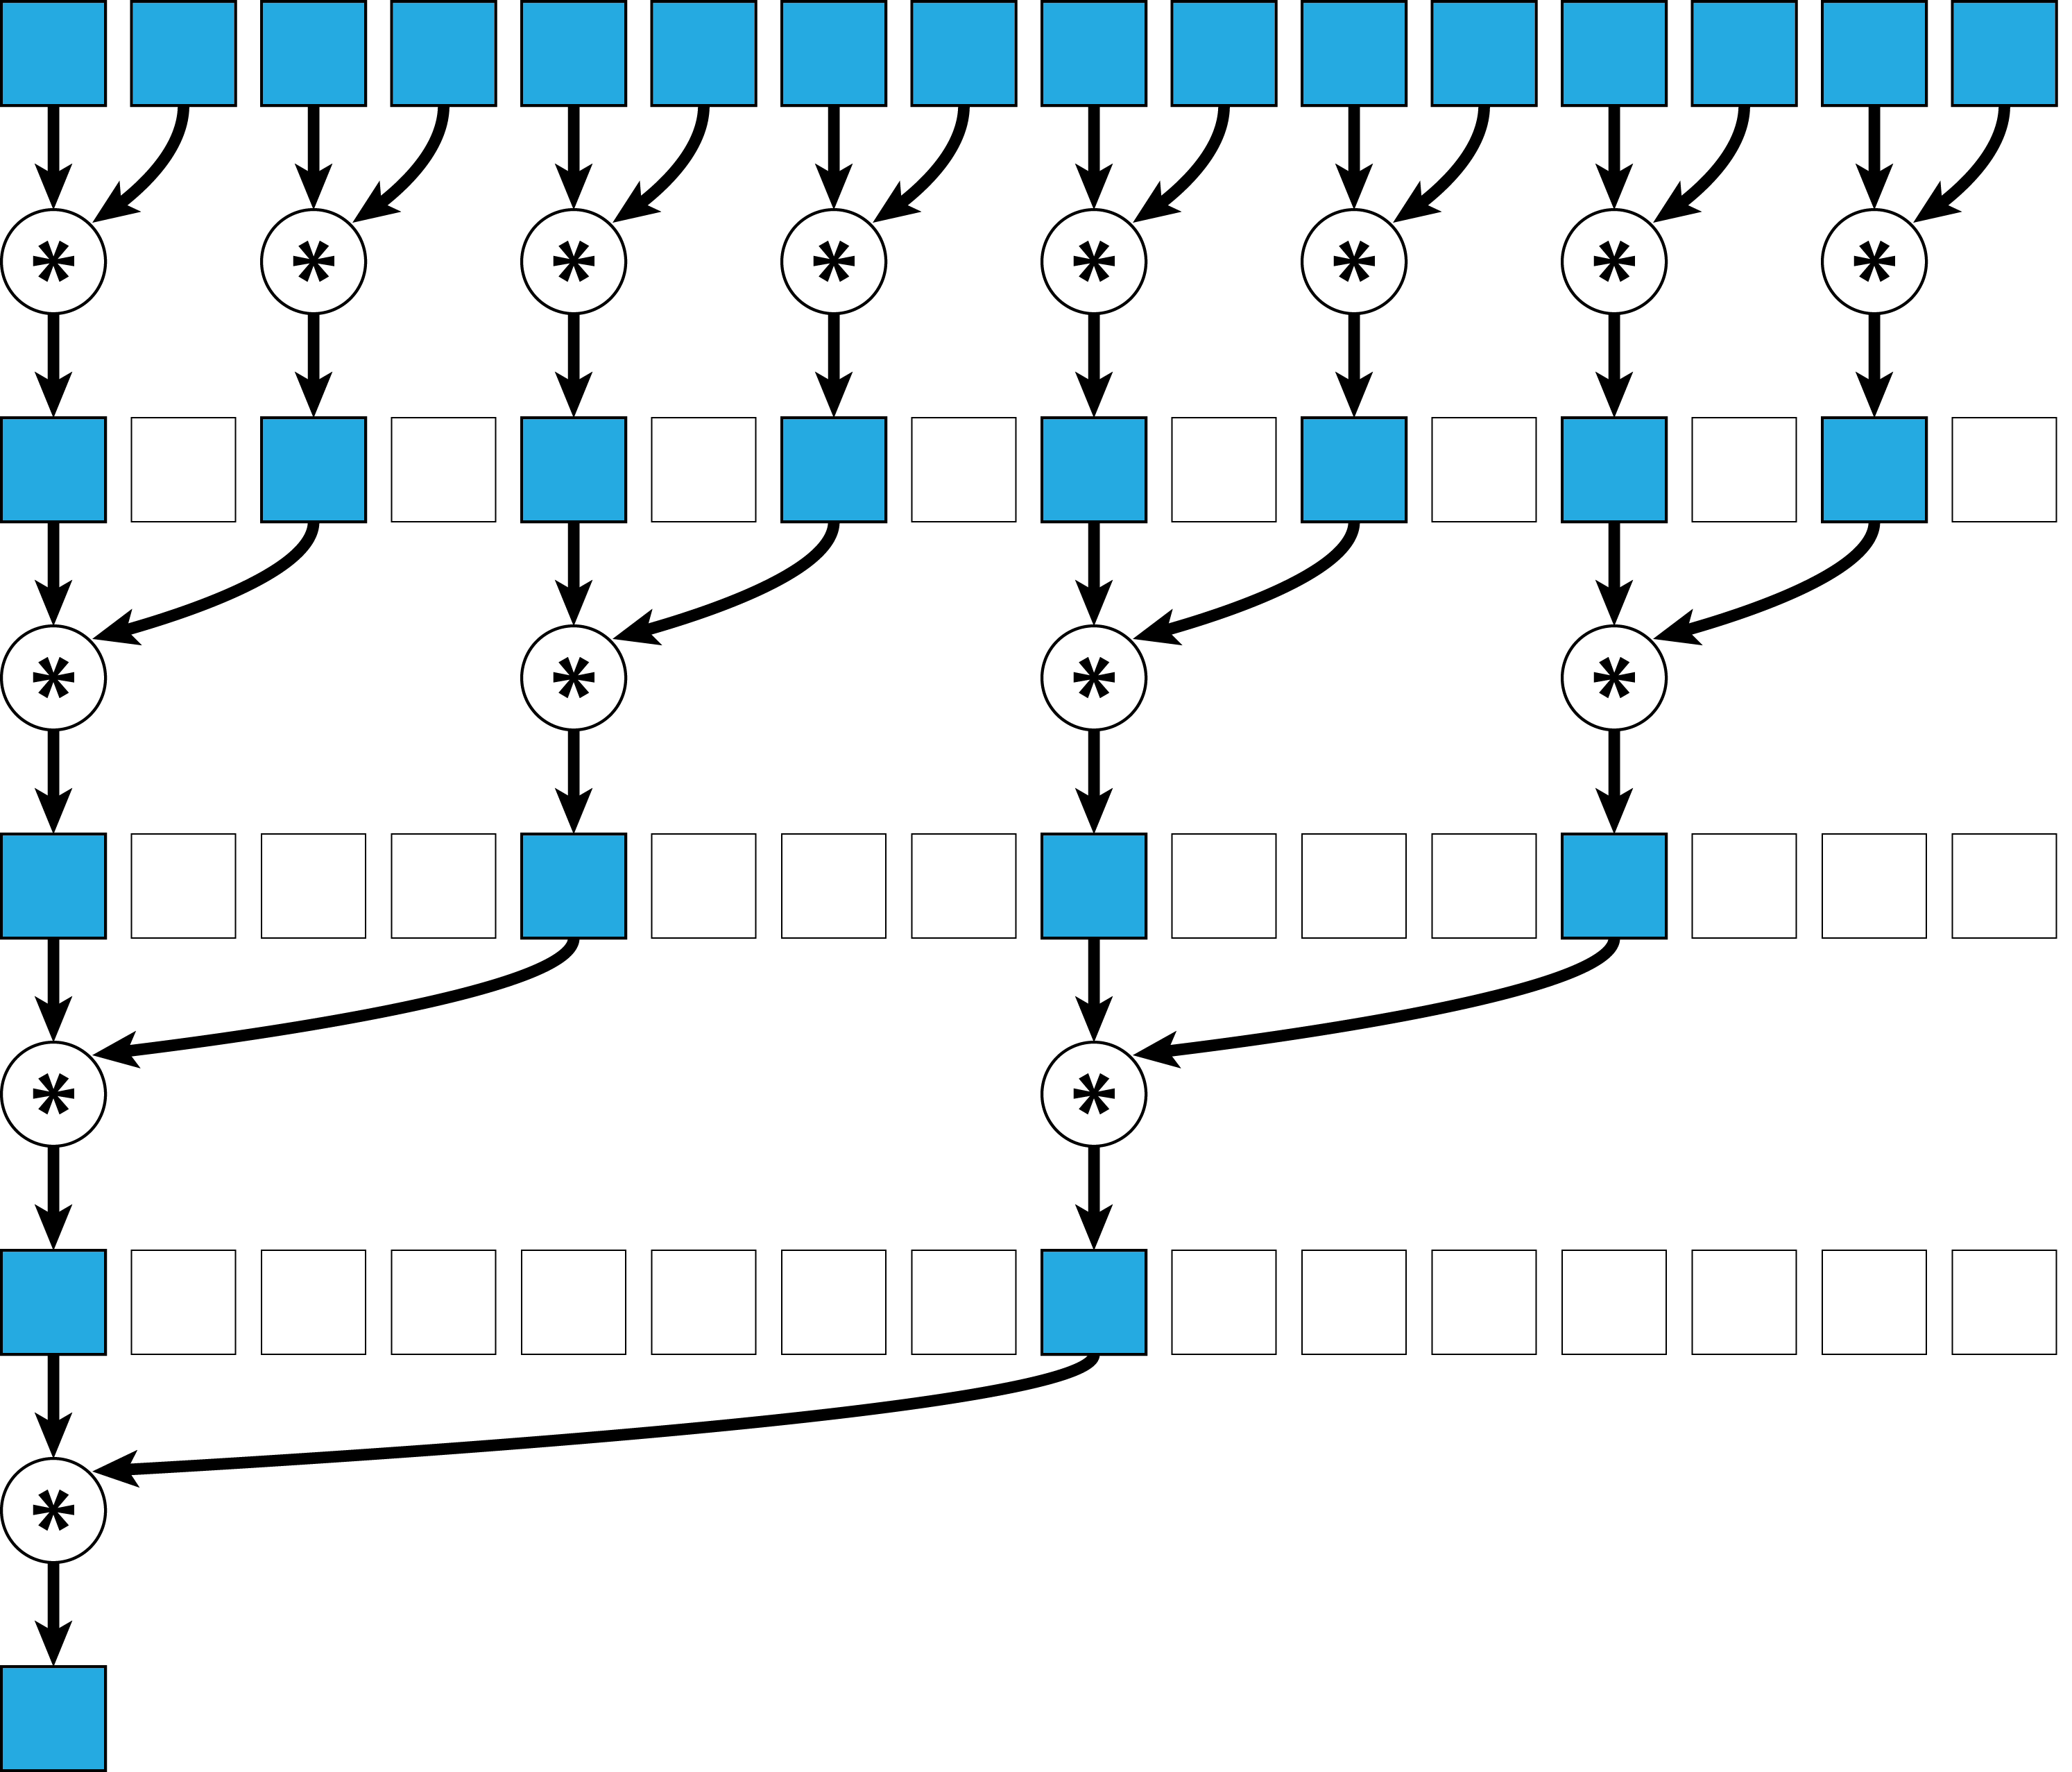
\includegraphics[width=10cm]{/images/parallelReduction.png}
    \captionof{figure}{Parallel reduction scheme}
\end{center}
\begin{verbatim}
int localMin = minWithVt(
    minimumValues[index],
    minimumValues[index + stride],
    Vt[minimumIndexes[index]],
    Vt[minimumIndexes[index + stride]]
);

int localMinIndex = minIndexWithVt(
    minimumValues[index],
    minimumValues[index + stride],
    minimumIndexes[index],
    minimumIndexes[index + stride],
    Vt[minimumIndexes[index]],
    Vt[minimumIndexes[index + stride]]
);
\end{verbatim}
The two functions above are responsible for finding the minimum and the minimum index, taking the corresponding Vt values into account.
This part of the implementation has been particularly tricky, with the algorithm not converging to a solution, due to set errors of the new Vt value.\\

At the end of the parallel reduction section there will be the value and the index of the minimum edge respectiverly at minimumValues[0] and minimumIndexes[0].

The update of the l array is executed in the same way as before, with every thread updating its cell of the array.\\

\subsubsection{Algorithm limitations}

The main setback of this algorithm is that it does not scale well with the number of nodes in the graph. In this case the tests were performed on a GPU with
a maximum number of thread per block of 1024, so that is the limit of the graph dimension. The performance evaluation is therefore not exhaustive due to the fact that the graph can
only be that big, a more powerful card should be able to handle bigger graphs and show the improvements in performance.\\

To make this algorithm usable on a GPU like the tested one, the usage of the shared memory should be completely eliminated,
because in that case the informations have to be available to threads which are not in the same block.

This would reduce the performances of the memory accesses, but would make the procedure available for lower end cards.\\

\newpage
\section{Benchmarking}

The tests have been performed on a machine equipped with a GPU NVidia GeForce GTX 1050 and an Intel processor i5-8300H with core frequency of 2.3 GHz,
the GPU architecture possesses these basic specifications:\\

\begin{itemize}
    \item   Max Threads per Block: 1024
    \item   Max Blocks per Multiprocessor: 32
    \item   Max Shared Memory size per Block: 49152 bytes\\
\end{itemize}

The performances in terms of execution time have been summarized into the following chart:

\begin{center}
    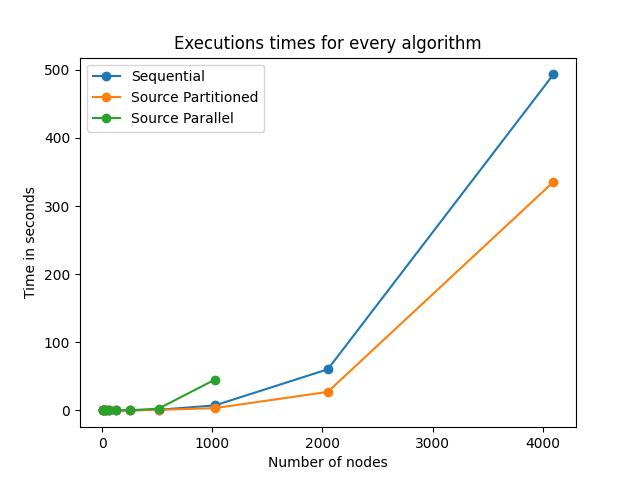
\includegraphics[width=12cm]{/images/chart.jpg}
    \captionof{figure}{Parallel reduction scheme}
\end{center}

The chart shows that the basic parallel version has a slighlty less tilted curve than the sedquential one, but the gain is not
that significant, while the improved parallel version shows an initial spike before the aother two starts to ascend. \\

This may be due to the overhead of the parallel execution, in an area where the number of nodes is not high enough to show its efficacy.
\newpage

The resulting speedups are the shown below:

\begin{center}
    \begin{tabular}{ |c|c|c| }
    \hline
    \textbf{Number of nodes} & \textbf{Basic parallel version} & \textbf{Improved parallel version} \\ \hline
    256 & 0.58  & 0.48 \\ \hline
    512 & 1.26 & 0.36 \\ \hline
    1024 & 2.18 & 0.16 \\ \hline
    2048 & 2.22 & NA \\ \hline
    4096 & 1.47 & NA \\ \hline
    \end{tabular}
\end{center}

The improved parallel version speedups could not be evaluated for graphs larger than 2014 nodes due to the testing machine
limitations. It is worth noting thought that the performances of the latter are always worse than the sequential version, while the basic
version outperforms the sequential starting from 512 nodes of dimensions. \\

All the speedups of the basic parallel version are evaluated considering a number of processors equal to the number of nodes, while the speedups
of the improved parallel version take into account $nodes * nodes$ processors.

\section{Conclusions}

This paper discussed about two parallel implementations of the Dijkstra's Algorithm, unfortunately the results cannot be cosidered conclusive in any way,
due to excessive testing limitations of the benchmarking machine. \\

The improved version performances are basically unknown at this point, because the testing could not work on graphs with a decent amount of nodes,
where the full parallel version would has the possibility to be effective compared to the other two versions. \\

The basic parallel version also does not show the expected speedup, while being faster than the sequential version the improvement shown does not bring the
time required to a smaller scale of reference, the elapsed time is smaller but in the same range of values. For this reason it is hard to tell if it would be worth using
parallel processors with this algorithm on a real problem, considering the costs of this type of hardware, for a gain that is not that significant. \\

\newpage
\printbibliography % Output the bibliography

%----------------------------------------------------------------------------------------

\end{document}